\documentclass[utf8x,show notes,pagenumber,hyperref={pagebackref=true,citecolor=green,bookmarks=true,pdfpagelabels=false}]{beamer} %remove draft when done with tex prep
%\documentclass[notes]{beamer} 
\usepackage{etex}
\usepackage{beamerthemesplit}
\usetheme{PaloAlto} %Hannover, Belin, Warsaw, PaloAlto, Frankfurt, Berkeley  etc

\usepackage{pgfpages}
\mode<handout>{\setbeamercolor{background canvas sidebar}{bg=red!45}}
\setbeamercolor{structure}{fg=gray}
\usepackage{bm}
\usepackage{subfloat}
\usepackage{paralist}
\usepackage{subcaption}
\usepackage{amssymb, amsmath}
\usepackage[round]{natbib}
\usepackage{algorithm}
\usepackage{algpseudocode}
\bibliographystyle{unsrtnat}
\usepackage[export]{adjustbox}
\usepackage{array,booktabs,tabularx}
\usepackage{tikz}
\usetikzlibrary{shapes,arrows, circuits, patterns, snakes, decorations.pathreplacing}
\usepackage{schemabloc, verbatim}
\usepackage{graphicx}
%\graphicspath{../}  % path to base directory of all papers
\DeclareGraphicsExtensions{.eps}

\usepackage{media9} % for video embeddings
\usepackage{multimedia} % for video embeddings
\usepackage{tcolorbox}
\tcbuselibrary{theorems}
\newcommand{\tcb}[2]
{
 \begin{tcolorbox}[title=\text{#2}]
 #1
 \end{tcolorbox}
}

%\renewcommand\thefootnote{}\footnote{#1}
\definecolor{light-blue}{rgb}{0.30,0.35,1}
\definecolor{light-green}{rgb}{0.20,0.49,.85}
\definecolor{purple}{rgb}{0.70,0.69,.2}

\newcommand{\lb}[1]{\textcolor{light-blue}{#1}}
\newcommand{\bl}[1]{\textcolor{blue}{#1}}

\newcommand{\maybe}[1]{\textcolor{gray}{\textbf{MAYBE: }{#1}}}
\newcommand{\inspect}[1]{\textcolor{cyan}{\textbf{CHECK THIS: }{#1}}}
\newcommand{\more}[1]{\textcolor{red}{\textbf{MORE: }{#1}}}

% FYA
\newcommand{\cmt}[1]{{\footnotesize\textcolor{red}{#1}}}%{#2}
%\newcommand{\note}[1]{\cmt{Note: #1}}
%\newcommand{\todo}[1]{\textcolor{cyan}{TO-DO: #1}}
\newcommand{\review}[1]{\noindent\textcolor{red}{$\rightarrow$ #1}}
\newcommand{\response}[1]{\noindent{#1}}
\newcommand{\stopped}[1]{\color{red}STOPPED HERE #1\hrulefill}

%Text commands
\newcounter{mnote}
\newcommand{\marginote}[1]{\addtocounter{mnote}{1}\marginpar{\themnote. \scriptsize #1}}
\setcounter{mnote}{0}
% \newcommand{\comment}[1]{}
\newcommand{\ie}{$i.e.$\ }
\newcommand{\eg}{e.g.\ }
\newcommand{\cf}{c.f.\ }
\newcommand{\yes}{\checkmark}
\newcommand{\no}{\ding{55}}

%Reference commands
\newcommand{\flabel}[1]{\label{fig:#1}}
\newcommand{\seclabel}[1]{\label{sec:#1}}
\newcommand{\tlabel}[1]{\label{tab:#1}}
\newcommand{\elabel}[1]{\label{eq:#1}}
\newcommand{\alabel}[1]{\label{alg:#1}}
\newcommand{\fref}[1]{\cref{fig:#1}}
\newcommand{\sref}[1]{\cref{sec:#1}}
\newcommand{\tref}[1]{\cref{tab:#1}}
\newcommand{\eref}[1]{\cref{eq:#1}}
\newcommand{\aref}[1]{\cref{alg:#1}}

\newcommand{\bull}[1]{$\bullet$ #1}
\newcommand{\argmax}{\text{argmax}}
\newcommand{\argmin}{\text{argmin}}
\newcommand{\mc}[1]{\mathcal{#1}}
\newcommand{\bb}[1]{\mathbb{#1}}


\def\tidx{t}
%\def\comment
%\def\value{V}
% from https://www.cs.jhu.edu/~jason/advice/write-the-paper-first.html
\newcommand{\Note}[1]{}
\renewcommand{\Note}[1]{\hl{[#1]}}  % comment out this definition to suppress all Notes
%\algnewcommand\algorithmicforeach{\textbf{for each}}
%\algdef{S}[FOR]{Foreach}[1]{\algorithmicforeach\ #1\ \algorithmicdo} %

%\newcolumntype{M}[1]{>{\centering\arraybackslash}m{#1}}
\def\coriolis{\textbf{\textit{C}}}
\def\massinertia{\textbf{\textit{M}}}
\def\torque{\bm{\tau}}
\def\frictionvec{\textbf{\textit{f}}}
\def\Smat{\textbf{\textit{S}}}
\def\Bmat{\textbf{\textit{B}}}
\def\wheelrad{\textbf{\textit{r}}}

\def\stateweight{\textbf{\textit{w}}_x}
\def\actionweight{\textbf{\textit{w}}_u}
\def\advactionweight{\textbf{\textit{w}}_v}

%Thesis defs
%\def\upchi{\textchi}
\def\kau{\mc{K}}
\def\particle{\bm{x}}
\def\deformationgrad{\textbf{F}}
\def\refconf{\bm{\upchi}_0}
\def\refconfbody{\mathscr{B}_0}
\def\conf{\bm{\upchi}}
\def\currconf{\bm{\upchi}}
\def\Eulerian{\mc{E}}
\def\cauchystress{\bm{\sigma}}
\def\stresscomp{\sigma}
\def\currconfbody{\mathscr{B}}
\def\materialresponse{\textbf{G}}
\def\orthoggroup{{\textit{SO}}(3)}
\def\liegroup{{\textit{SE}}(3)}
\def\liealgebra{\mathfrak{se}(3)}
\def\identity{\textbf{I}}
\newcommand{\trace}[1]{\textbf{tr}(#1)}
\def\leftcauchy{\textbf{B}}
\def\rightcauchy{\textbf{C}}
\def\fiber{\textbf{dx}}

\def\dof{\text{DOF }}
\def\dofs{\text{DOFs }}
\def\reline{\mathbb{R}}
\def\curve{\deformationgrad}
\def\twist{{\xi}}
\def\contactforce{\tilde{F}}
\def\contactforcecomp{f}
\def\gaussianmap{\textbf{}n}
\def\contacttorquecomp{\tau}
\def\wrt{with respect to }
\def\curveparam{\position}
\def\basis{\bm{e}}
\def\pose{{g}}
\def\selmap{{B}}
\def\manipmap{{G}}
\def\jacob{\bm{J}}
\def\normal{\bm{n}}
\def\position{\textbf{r}}
\def\deformationgradcur{\textbf{H}}
\def\eulerianvel{\textbf{v}(\position, t)}
\def\headparam{\zeta}
\def\strain{\mathrm{\Psi}}
\def\strainiso{\mathrm{\Psi_{\text{iso}}}}
\def\strainfiber{\mathrm{\Psi_{\text{mesh}}}}

% mechanism defs
\def\wallthickness{1cm}
\def\sorodiam{9 cm}
\def\sorodiamdim{5-6.25cm}

% inline macros
\newcommand{\putsoro}[2]{\includegraphics[width=.45\columnwidth,height=#2\columnwidth]{../../../PhDThesis/figures/#1}}
\newcommand{\sorowidth}{.35}


%\newtheorem{theorem}{Theorem}[]
%\newtheorem{example}{Example}
%\newtheorem{homework}{Homework}

\tikzstyle{block} = [draw, fill=yellow!80, rectangle,minimum height=3em, minimum width=4em]
\tikzstyle{sum} = [draw, fill=white!20, circle, node distance=1cm]
\tikzstyle{input} = [coordinate]
\tikzstyle{output} = [coordinate]
\tikzstyle{pinstyle} = [pin edge={to-,thin,black}]

\newcolumntype{Z}{>{\centering\arraybackslash}X} % centered tabularx columns
\newcommand{\pphantom}{\textcolor{ta3aluminium}} % phantom
%\setbeamerfont{title}{shape=\itshape,family=\rmfamily}
\setbeamercolor{title}{fg=magenta!70!black,bg=yellow!70!white}
%
\title{\small A short treatise on robots' geometry, kinematics, and dynamics.}

\author{Author: Lekan Molu}
\institute{
	%
	\vspace{0.5em}
	%
	Dissemination: Microsoft Research RL Group, \\
	New York City, NY 10012 
}

\date{\today} 


\setbeamersize{sidebar width left=2cm}
%remove title and author names from sidebar
  \makeatletter
\setbeamertemplate{sidebar \beamer@sidebarside}%{sidebar theme}
{
	\beamer@tempdim=\beamer@sidebarwidth%
	\advance\beamer@tempdim by -6pt%
	\insertverticalnavigation{\beamer@sidebarwidth}%
	\vfill
	\ifx\beamer@sidebarside\beamer@lefttext%
	\else%
	\usebeamercolor{normal text}%
	\llap{\usebeamertemplate***{navigation symbols}\hskip0.1cm}%
	\vskip2pt%
	\fi%
}%
\makeatother

\begin{document}
	\maketitle
%http://tug.ctan.org/macros/latex/contrib/beamer/doc/beameruserguide.pdf#subsection.21.3
\begin{frame}
	\frametitle{Table of Contents}
	\tableofcontents[pausesections]
\end{frame}

\chapter{Preamble}
\label{chap:intro}

Consider this your roadmap for the course.  Please read through the syllabus posted on moodle carefully and feel free to share any questions that you may have.  Please print a copy of the syllabus for reference. Some relevant parts of the syllabus are repeated here but the moodle reference should serve as your guide throughout the ten weeks of this course.

\section{Course Description}
This course focuses on the algorithmic and mathematical concepts  with respect to robot planning, manipulation and control. Topics covered include kinematics and dynamics, as well as path planning and deep reinforcement learning algorithms. Simulations and experiments on hardware testbeds (listed in the syllabus) will be performed to test the related algorithms.

\section{Course Outcomes}
After taking this course, each student will be able to

\begin{itemize}
\item Develop planning and manipulation schemes to drive robot operation

\item Integrate perception algorithms into manipulation and planning systems

\item Determine the kinematic description of a robot's motion or locomotion
\end{itemize}

\section{Prerequisites}

RBOT 210 or an advanced knowledge of ROS; undergraduate-level experience or equivalent with object oriented programming; strong programming knowledge in Python and C++ is required; and RBOT 205 if mathematical foundational skills of admissions criteria are needed.

\section{Recommended Texts}
\begin{itemize}
	\item  	Main Texts
	\begin{itemize}
		\item Murray, R. M., Li, Z., and Sastry, S. S. (1994). A Mathematical Introduction to Robotic Manipulation. Book (Vol. 29). Free PDF preprint downloadable from, \href{https://www.cds.caltech.edu/~murray/books/MLS/pdf/mls94-complete.pdf }{Murray's website}.
		%
		\item 	Spong, M. W., Hutchinson, S., and Vidyasagar, M. (2012). Robot Modeling and Control. Students can buy from this \href{https://www.amazon.com/Robot-Modeling-Control-Mark-Spong/dp/0471649902}{Amazon Link}.
	\end{itemize} 
	%
	\item Secondary Text
	%
	\begin{itemize}
		\item Modern Robotics: Mechanics, Planning, and Control. Free PDF preprint downloadable from \href{ http://hades.mech.northwestern.edu/images/7/7f/MR.pdf}{Author's Northwestern Website}.		
	\end{itemize} 
    %
    \item 
    Auxiliary Text: 
    %
    \begin{itemize}
    	\item Theory of Screws: A Study in the Dynamics of a Rigid Body by Robert Stawell Ball, Dublin: Hodges, Foster, and Co., Grafton-Street (Should be downloadable via Interlibrary Loan).
    \end{itemize}
\end{itemize}

\section{Recommended Journals}
	%
	\begin{itemize}
		\item 
		\href{ https://ieeexplore.ieee.org/xpl/RecentIssue.jsp?punumber=8860}{IEEE Transactions on Robotics}.
		%
		\item 
		\href{https://journals.sagepub.com/home/ijr}{The International Journal of Robotics Research}.
		%
		\item 
		\href{https://www.ieee-ras.org/conferences-workshops/fully-sponsored/icra}{The IEEE International Conference on Robotics and Automation}.
		%
		\item \href{https://www.ieee-ras.org/conferences-workshops/financially-co-sponsored/iros}{IEEE/Robotics Society of Japan International Conference on Intelligent Robots and Systems (IROS)}.
		%
		\item \href{https://www.journals.elsevier.com/robotics-and-autonomous-systems}{Robotics and Autonomous Systems, An Elsevier Journal}.
	\end{itemize}

\section{Required Software}
	
	\begin{itemize}
	%
	\item A working knowledge of python and the anaconda environment.
	%
	\item \href{https://www.ros.org/}{The Robot Operating System}.
	%
	\item ROS from Conda installation \href{ https://medium.com/@wolfv/ros-on-conda-forge-dca6827ac4b6}{instructions}.
	\end{itemize}

\section{Online Course Content}
%
This course will be conducted completely online using Brandeis’ LATTE \href{http://moodle2.brandeis.edu}{site}. The site contains the course syllabus, assignments, our discussion forums, links/resources to course-related professional organizations and sites, and weekly checklists, objectives, outcomes, topic notes, self-tests, and discussion questions.  Access information is emailed to enrolled participants before the start of the course.   To begin participating in the course, review the ``Welcoming Message" and the ``Week 1 Checklist."

\section{Assessments and Labs}

Please read the syllabus posted on the RBOT 250 website thoroughly.

\section{Errata}

If in the course of using these notes, you find sentence errors, errata or mistakes in equations, please annotate them and upload it to the discussion forum. Points will awarded, at the discretion of the instructor, for such help.
\section{Mechanisms}

\begin{frame}
	\frametitle{Topics}
	\begin{tcolorbox}[coltitle=yellow!50!black,colframe=magenta!25,split=.2,title=Mechanism Components]
		Freedoms, Constraints, and Mobility.
		\tcblower
		%\begin{itemize}
		 Kinematic Geometry: Pairs, linkages, and mechanisms.
		 \vspace{.2cm}
		\newline
		Motion of linkages: Screws, and spatial motions.
		\vspace{.2cm}
		\newline
		Freedom and Mobility: Freedoms, unfreedoms, connectivity, mobility;
		\vspace{.2cm}
		\newline
		Gr{\"u}bler-Kutzbach's mobility criterion and examples.
	\end{tcolorbox}
\end{frame}
 
\begin{frame}
	\frametitle{Definition of a Mechanism}
		\begin{definition}[Lekan Molu]
			A \textcolor{blue}{connection} of  mechanical, magnetic, electrical, hydraulic, or pneumatic components forming an \textcolor{magenta}{assemblage}, meant for moving rigid, semi-rigid or non-rigid bodies via a \textcolor{green}{controlled generation} of \textcolor{red}{motion}.
		\end{definition}
		%
	\begin{tcolorbox}[coltitle=red!80!black,colframe=magenta!25,title=Kenneth Hunt (1978)]
			A means of \textit{transmitting}, \textit{controlling}, or \textit{constraining} the relative movement.
	\end{tcolorbox}
\end{frame}

\begin{frame}
	\frametitle{Mechanisms}
	\begin{block}{Joints and links}
		Joints are a result of the connecting points between rigid links.
		Links may be rigid mechanical parts, elastic, (vulcanized) rubber components, diaphragms, conveyor belts, spring-damper systems e.t.c.
	\end{block}
	%	
	\begin{block}{Rigid Mechanism}
		Our chief focus will be rigid links, \textcolor{red}{pairs}, components and mechanisms in general.
	\end{block}
\end{frame}


\begin{frame}
	\frametitle{Mechanisms Examples}
	\begin{tabular}{|c|c|} 
	%
	\hline  \\
	Spring-Mass-Damper System & Excavator \\
	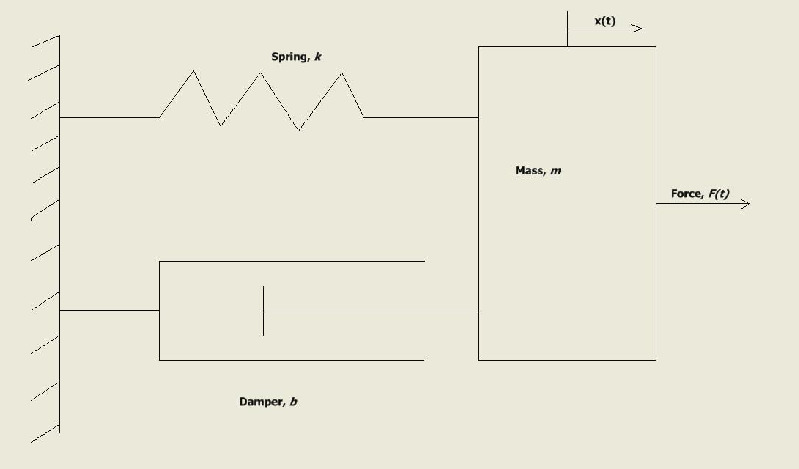
\includegraphics[height=5em,width=10em]{figures/spring-mass-damper.jpg} & 
	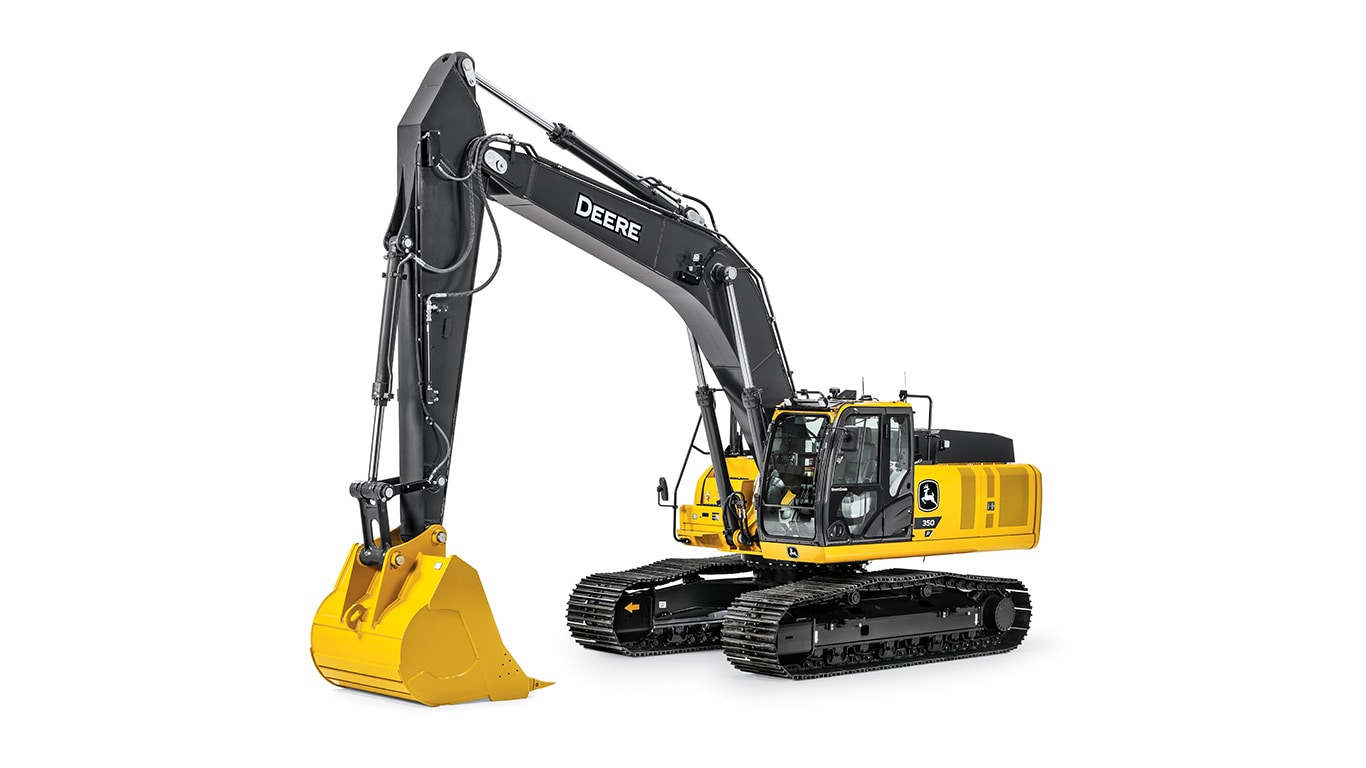
\includegraphics[height=5em,width=10em]{figures/excavJohnDeere.jpg} \\
	\hline \\
	Car suspension & Daimler  Plant \\
	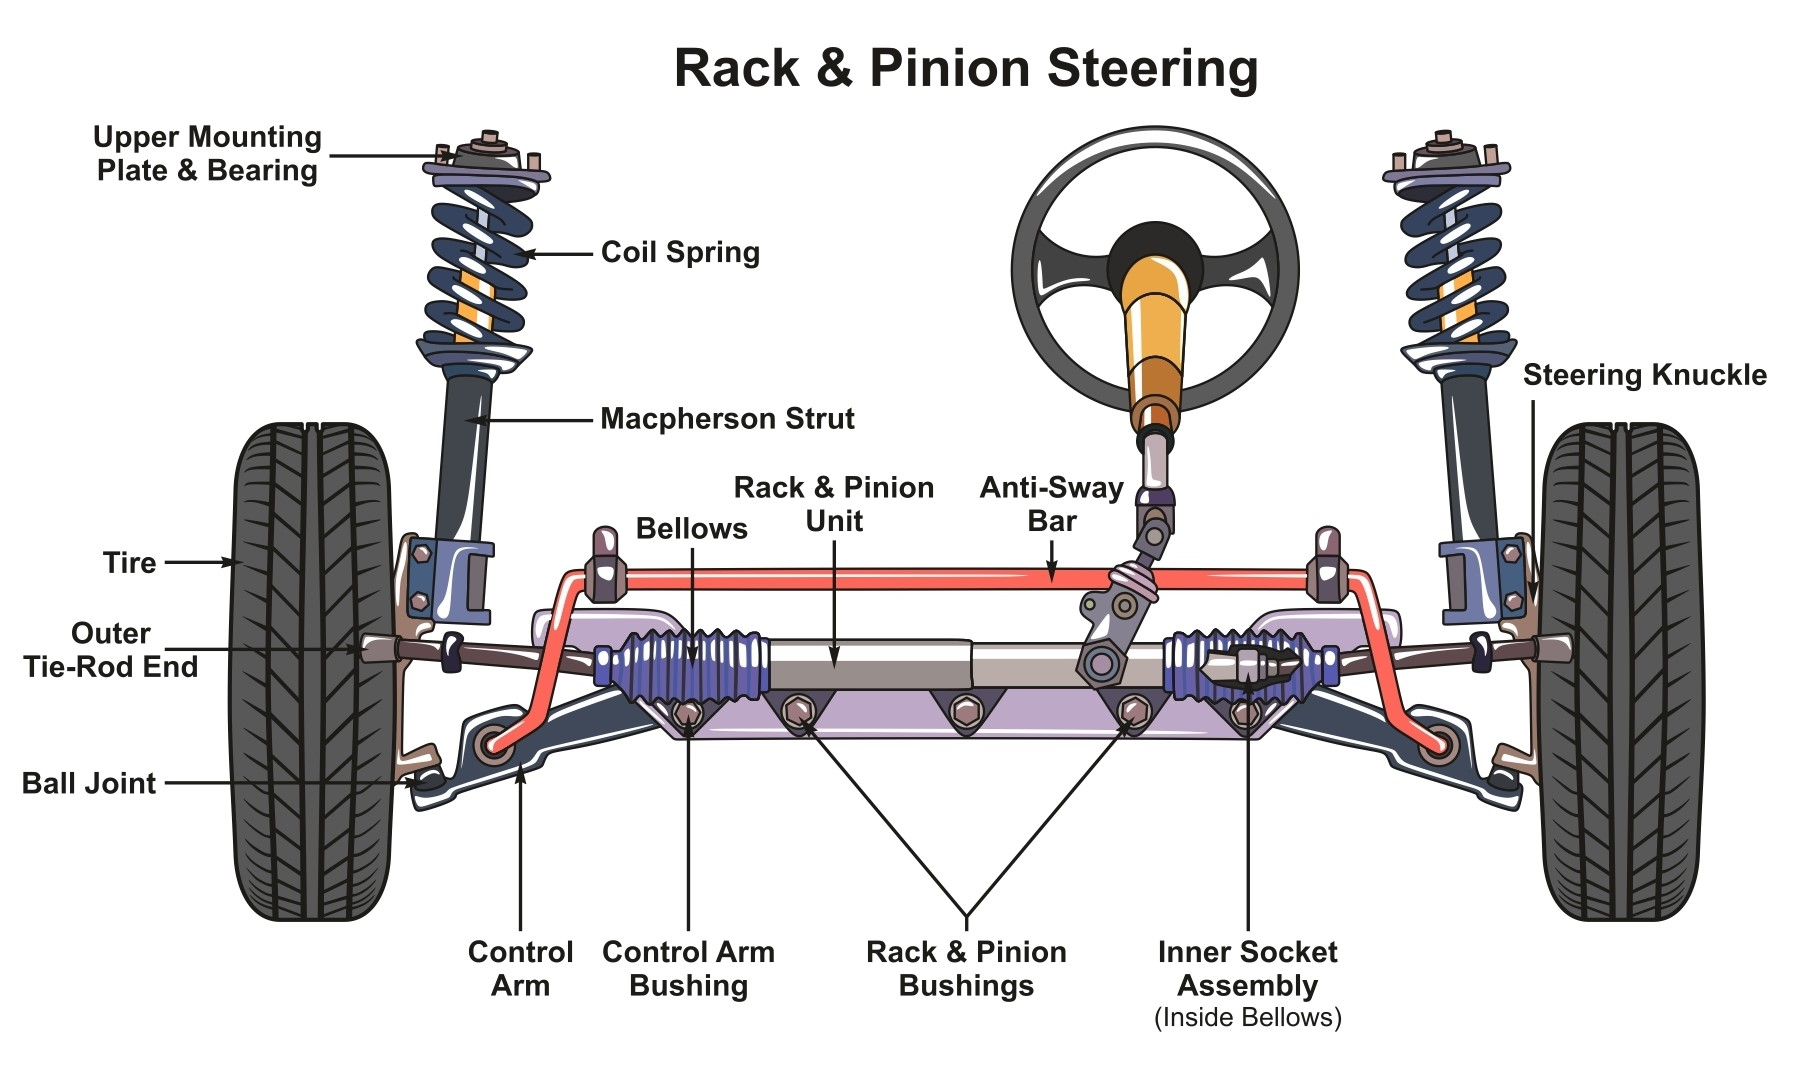
\includegraphics[height=5em,width=10em]{figures/carsusp.jpg} &
	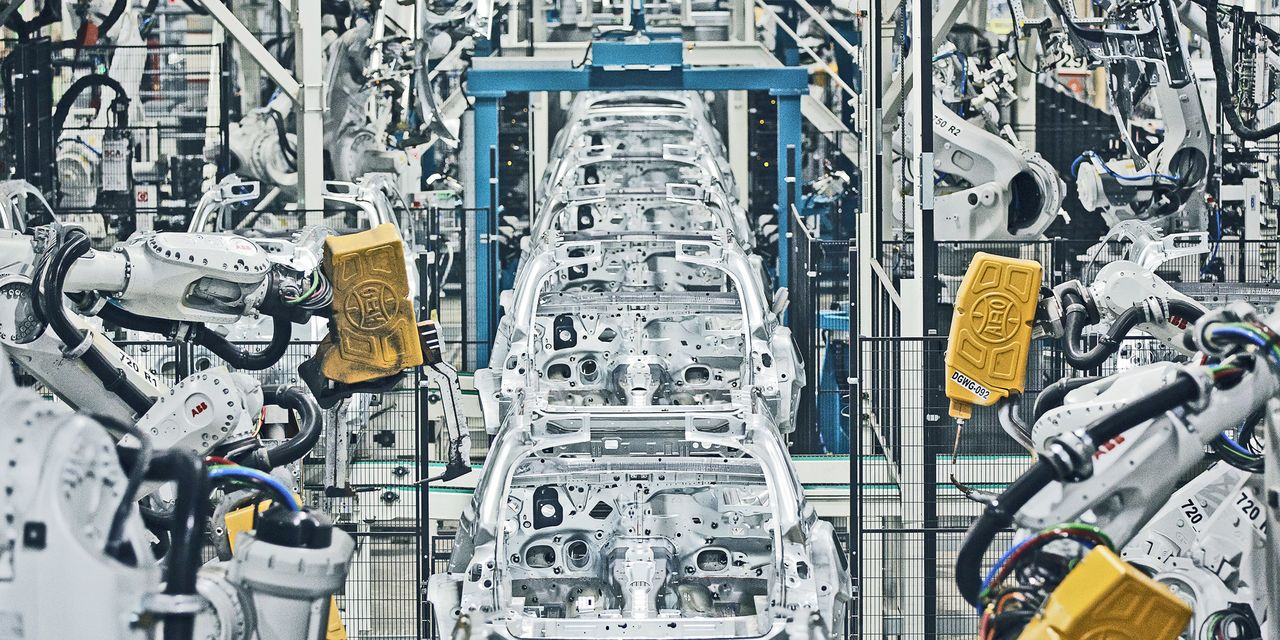
\includegraphics[height=5em,width=10em]{figures/daimler_manuf.jpeg} \\
	\hline
	\end{tabular}
\end{frame}

\note{The PUMA arm is the world's first serial kinematic chain. Developer: Victor Scheinman, Stanford student in the `50's. Made several iterations. Patent Rights: Joe Engelberger, (Danbury Unimation, 1961). Joe -- father of robotics -- created world's first robotics company in '61.}
\begin{frame}
	\frametitle{Robot Mechanisms}
	\begin{definition}[Ken Salisbury Jr., 1982]
		``\footnotesize \textit{[Robots are] our fascination with constructing mechanical analogues of ourselves... [this fascination] has led us to place all sorts of hopes and expectations in robot capabilities}."
	\end{definition}
	\begin{columns}[t]
		\begin{column}{5cm}
			\begin{minipage}[b]{.5\textwidth}
				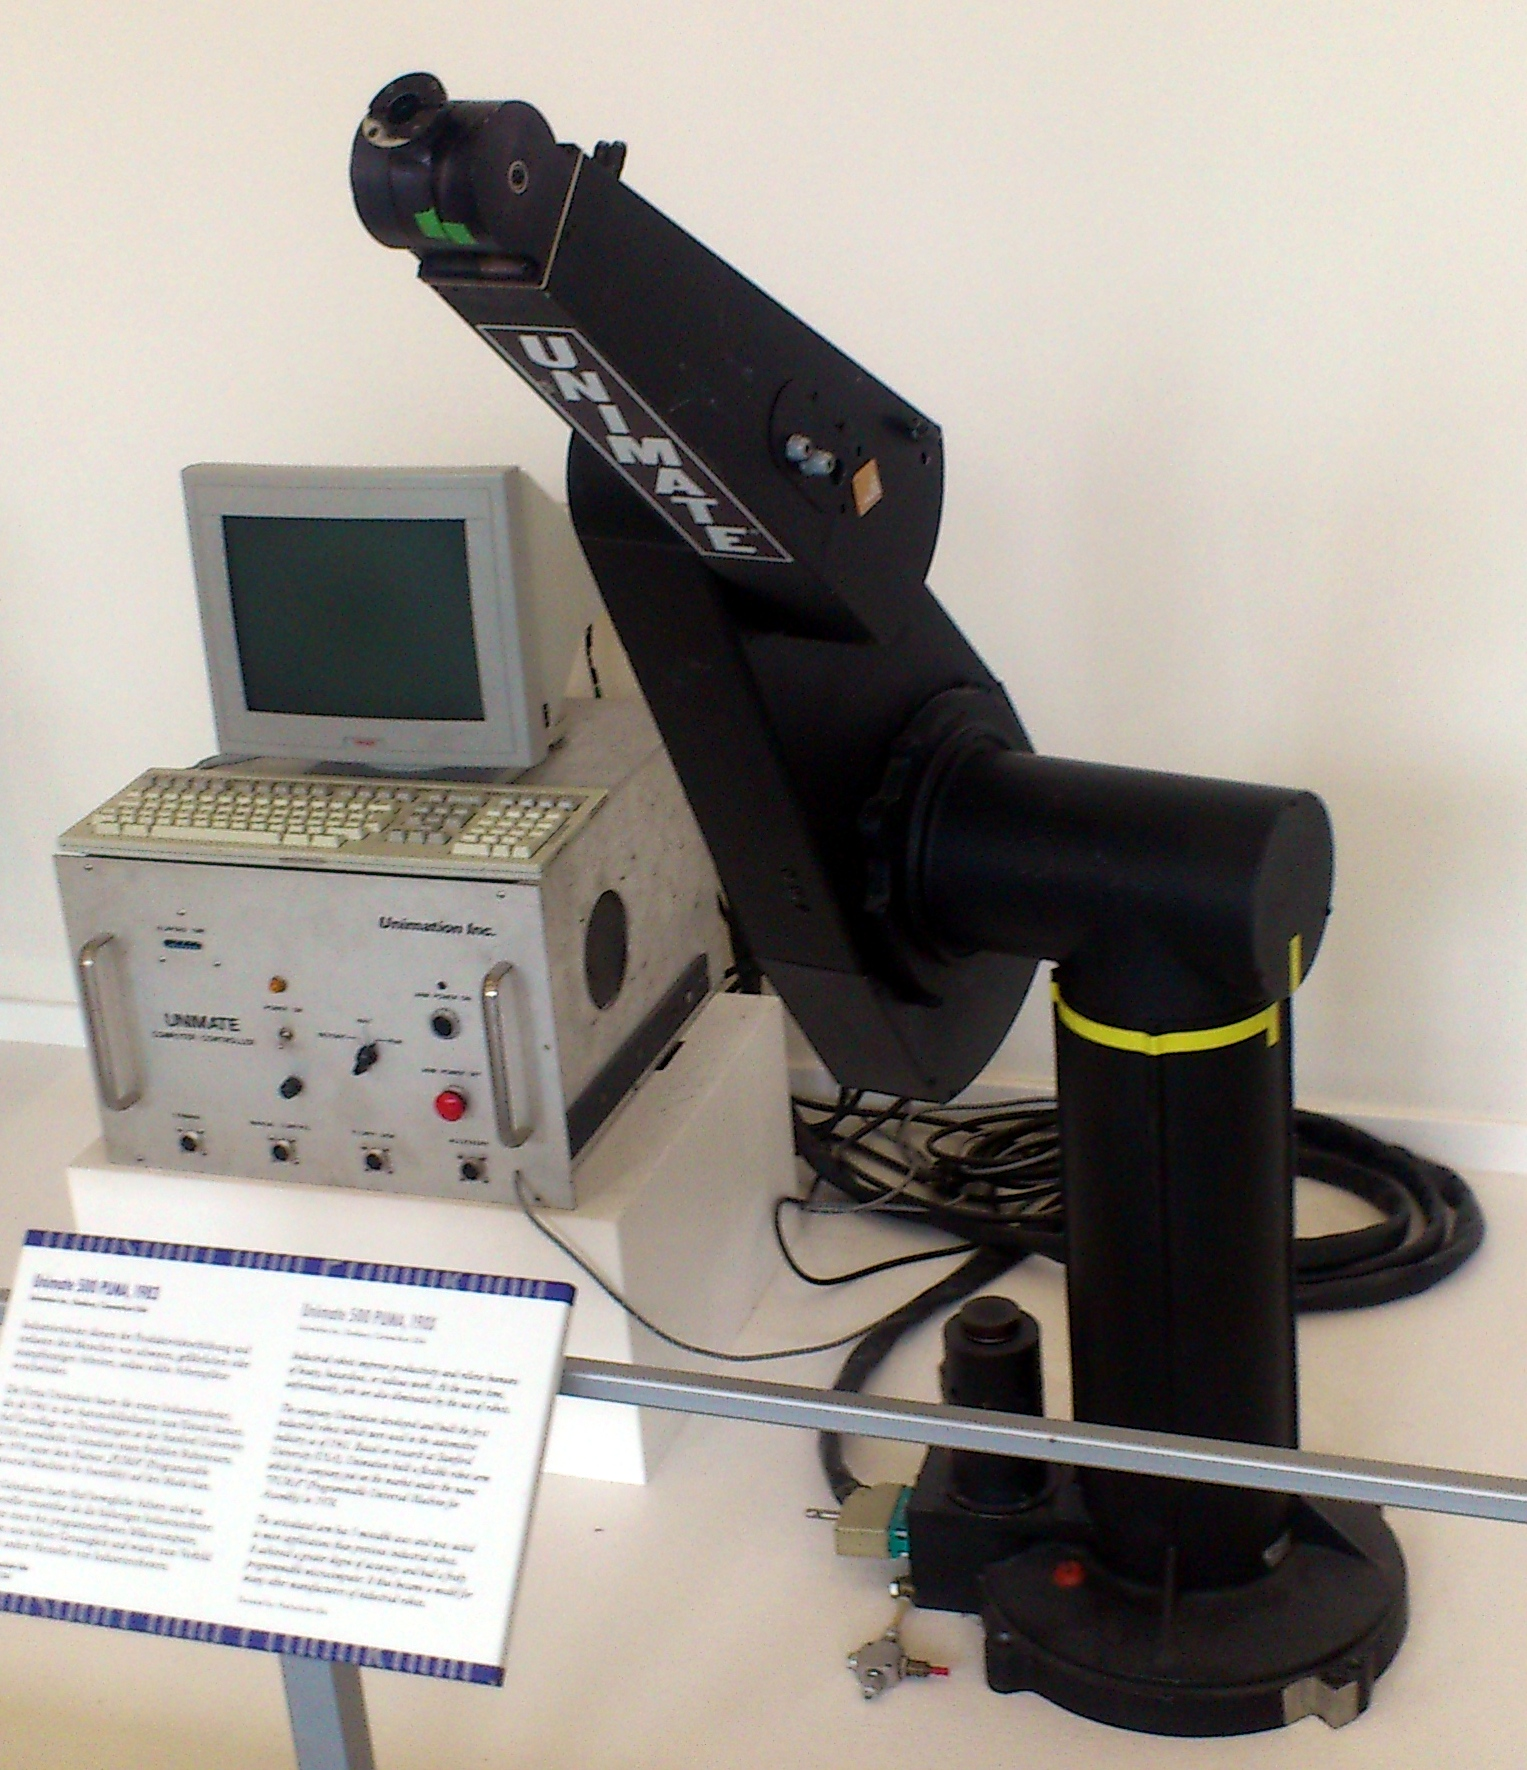
\includegraphics[width=1.5\textwidth, height=1.5\textwidth]{../Notes/figures/PUMA.jpg} \\
				\footnotesize{The St{\"a}ubli PUMA Robot (1956).} %Programmable Universal Manipulation Arm.}
		\end{minipage}
	%
	\end{column}	
		\begin{column}{5cm}
			\begin{minipage}[b]{.5\textwidth}
				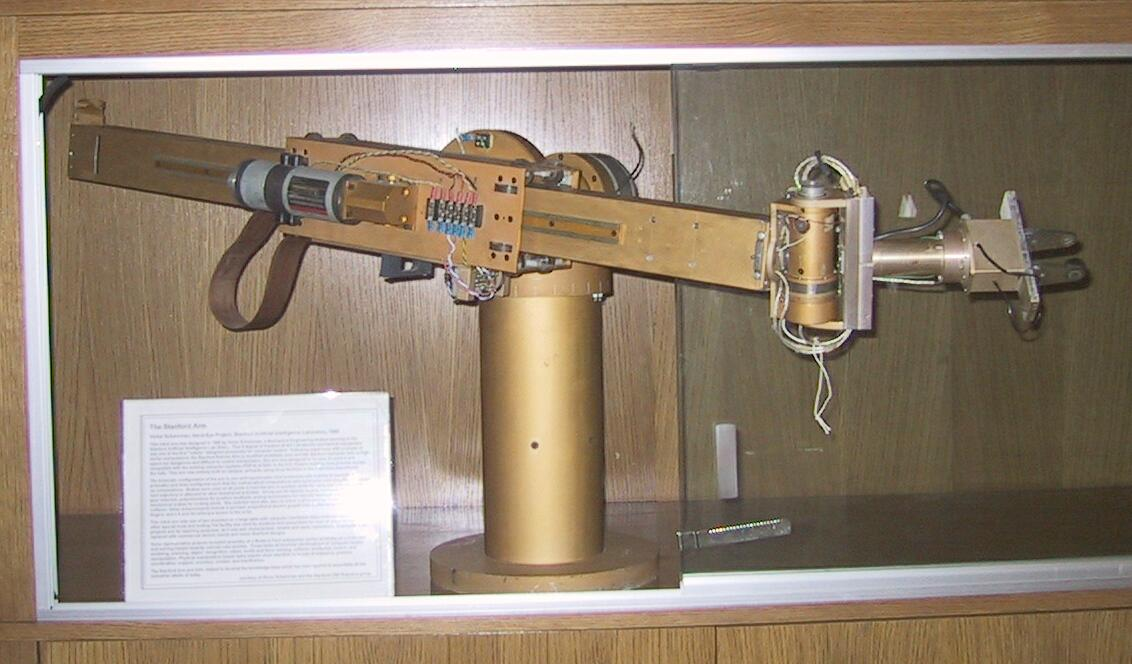
\includegraphics[width=1.5\textwidth, height=1.5\textwidth]{../Notes/figures/StanfordArm.jpg}  \\
				\footnotesize The Stanford Arm (Infolab 1969). %Six degrees of freedom open kinematic chain.
			\end{minipage}
		\end{column}
	\end{columns}
\end{frame}

\begin{frame}
	\frametitle{Long Walk Towards Direct Drive Robot Arms}
	
	\begin{tcolorbox}[coltitle=magenta!80!green,colframe=yellow!80!green]
		The 50's, 60's nd 70's witnessed use of hydraulics  for (feedforward) position control.
	\end{tcolorbox}
	
	\begin{tcolorbox}[coltitle=magenta!80!green,colframe=blue!80!green] 
		For feedback control, force sensors and pressure sensors were used in closed-loop scenarios.
	\end{tcolorbox}

	\begin{tcolorbox}[coltitle=magenta!80!green,colframe=red!80!green] 
		Electrical actuation meant that robots had to be operated at high speeds. Needs for gear reduction for safe operations at low speeds. 
	\end{tcolorbox}

	\begin{tcolorbox}[coltitle=magenta!80!green,colframe=brown!80!green]
		 With gear reduction came backlash, friction, and associated expense.
	\end{tcolorbox}
\end{frame}


\note{CMU DD I/II Arms: Workspace is donut shaped. OD:  90cm; ID: 21.7cm; $1.8m^2$ workspace area. Built by Harry Asada. Structural design similar to aircraft gimbal arm; Uses Samarium Cobalt rare earth magnet brushless DC motors on first 3 joints, and AlNiCo magnets on tip joints. No belts, transmissions making for faster transmitting of motions, less friction, low energy, low compliance. Each joint has complex AL housing which enables: (i) Control of geometrical relationships of bearing assembly; (ii) Control of servo components to bearing assembly; (iii) Controls of rotational axes to consecutive joints.}


\begin{frame}
	\frametitle{Direct Drive Robot Mechanism: CMU DD I Arm}
	\begin{columns}[t]	
		%
		\begin{column}{.45\columnwidth}
			\begin{minipage}[b]{\textwidth}
				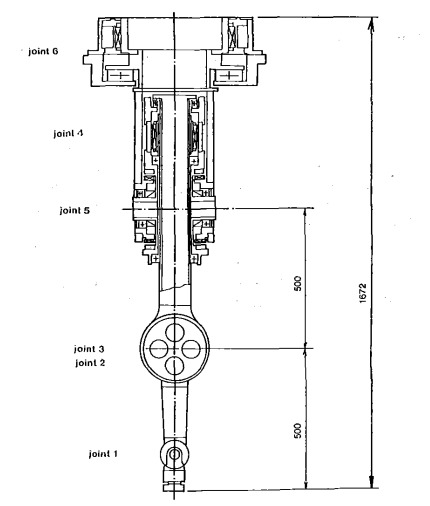
\includegraphics[width=1.2\textwidth, height=1.5\textwidth]{figures/cmu_arm.jpg} \\
				\footnotesize{Arm Schematics Transmission} %Programmable Universal Manipulation Arm.}
		\end{minipage}
		%
	\end{column}
	%
	\begin{column}{.45\columnwidth}
		\begin{minipage}[b]{\textwidth}
			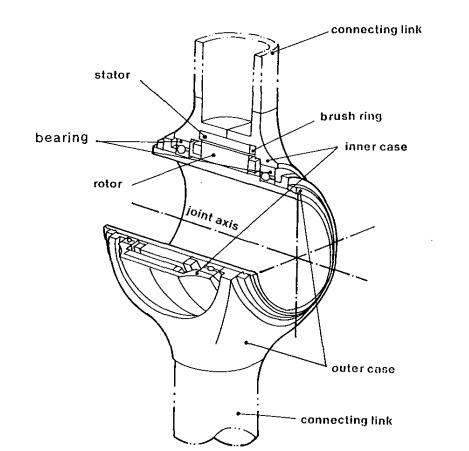
\includegraphics[width=1.2\textwidth, height=1.5\textwidth]{figures/dd_joints.jpg} \\
			\footnotesize{Joint schematic} %Programmable Universal Manipulation Arm.}
	\end{minipage}
	%
	\end{column}
\end{columns}
\end{frame}

\begin{frame}
	\frametitle{Direct Drive Robot Mechanism: CMU DD I Arm}
	\begin{columns}[t]					%
		%
		\begin{column}{.45\columnwidth}
			\begin{minipage}[b]{\textwidth}
				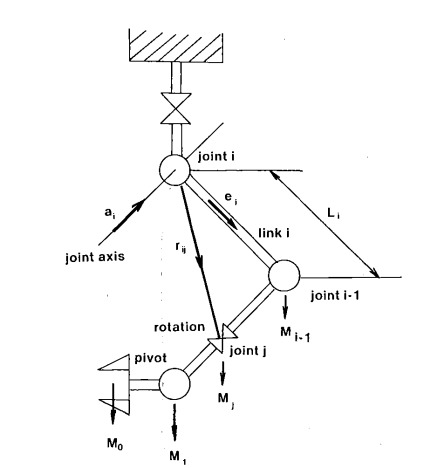
\includegraphics[width=1.1\textwidth, height=1.5\textwidth]{figures/dd_kinematics.jpg} \\
				\footnotesize{Kinematic model} %Programmable Universal Manipulation Arm.}
		\end{minipage}
		%
	\end{column}
				\begin{column}{.45\columnwidth}
					\begin{minipage}[b]{\textwidth}
						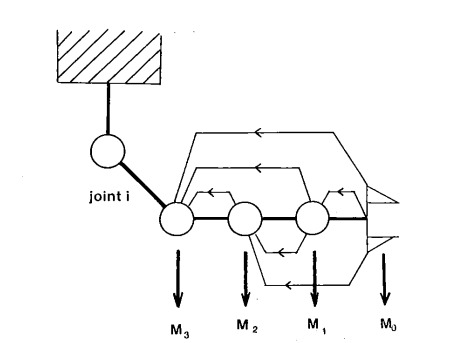
\includegraphics[width=1.2\textwidth, height=1.5\textwidth]{figures/dd_load_joints.jpg} \\
						\footnotesize{Errors Transmission} %Programmable Universal Manipulation Arm.}
				\end{minipage}
				%
			\end{column}
	\end{columns}
\end{frame}


\note{First direct-drive robot without a gearbox. Selective compliance in X-Y directions given its articulated jointed arms. One-freedom motion along $Z$ direction given its constrained arm New generations such as Cobra i600/i800 include power amplifiers, system and servo controls etc embedded in the robot's base. Kuka Scara arm: Lightweight, fast, powerful, low maintenance, energy consumption, investment costs etc.}
\begin{frame}
	\frametitle{Robot Mechanisms}
	\begin{columns}[t]	
		\begin{column}{5cm}
			\begin{minipage}[b]{.5\textwidth}
				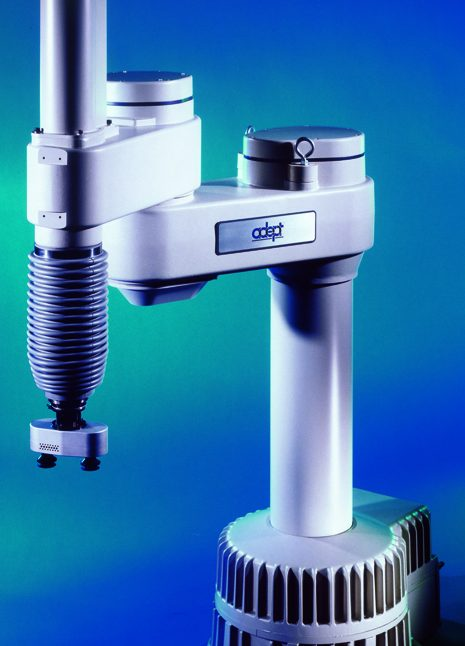
\includegraphics[width=1.5\textwidth, height=1.5\textwidth]{figures/adeptone.jpg}  \\
				\footnotesize The Adept One SCARA robot (Debuted 1984). 
			\end{minipage}
		\end{column}
		%
		\begin{column}{5cm}
			\begin{minipage}[b]{.5\textwidth}
				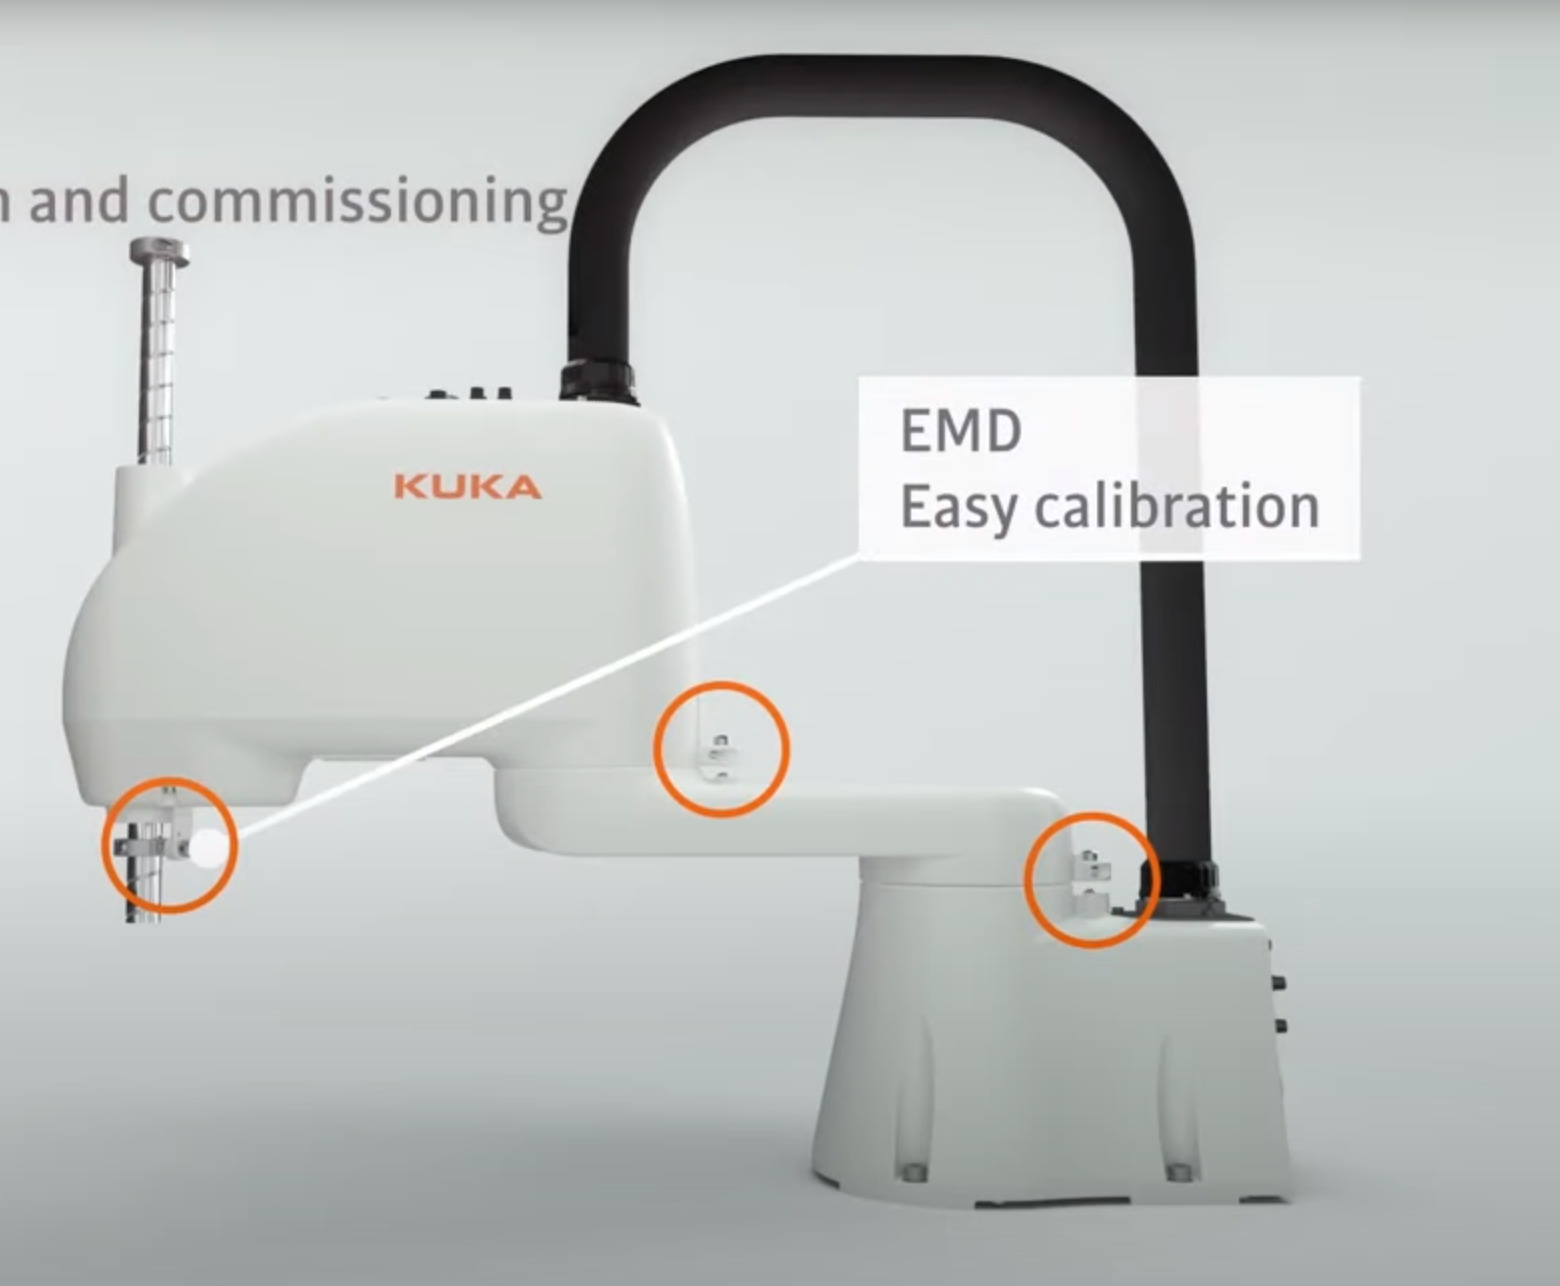
\includegraphics[width=1.5\textwidth, height=1.5\textwidth]{figures/Scara.jpg} \\
				\footnotesize{Kuka's SCARA arm, 2022. \copyright Kuka Robotics} %Programmable Universal Manipulation Arm.}
		\end{minipage}
		%
	\end{column}
\end{columns}
\end{frame}


\begin{frame}
	\frametitle{Open Kinematic Chains}
	%	
	\begin{block}{Chains}
		Open kinematic chains are based off the anthropomorphic construction of the human hand with cantilevered beam structures.
	\end{block}
%	\begin{description}
%		\item[The PUMA arm]  World's first serial kinematic chain 
%		\item [Developer:] Victor Scheinman, Stanford `50's
%		\item [Patent Rights:] Joe Engelberger, (Danbury Unimation, 1961).
%	\end{description}
	%
	\begin{block}{Chain Mechanism}
		 Amplifies errors from waist to tool frame. Control difficult. 
	\end{block}
	%
	\begin{block}{Control}
		Feedforward control: High power and precision hydraulic actuators for servo motors. \\
		Sensory feedback control: Force sensing (Ernst, 1962). 
	\end{block}
\end{frame}


\begin{frame}
	\frametitle{Open Kinematic Chains}
	%
	\begin{columns}[t]
		\begin{column}{.5\columnwidth}
			\begin{description}
				\item Unstructured environmental interaction;
				\item Project MAC, MIT;
				\item Tomovic and Boni's pressure sensed grasp;
				\item Binary robot vision system (McCarthy et al, 1963).
			\end{description}
		\end{column}
	\begin{column}{.5\columnwidth}
	\begin{description}
		\item Stanford Manipulator;
		\item Boston arm;
		\item The AMF (American Machines and Foundry) arm;
		\item General electric's walking robot (1969)
		\end{description}
\end{column}
	\end{columns}
\end{frame}

% ---- Bibliography ----
\bibliographystyle{../../Proposal/styles/bibtex/spmpsci_unsrt}
{
\tiny
\bibliography{../../../SRS/Continuum/biblio}
}
\end{document}
